\documentclass[11pt,oneside]{fithesis2}
\usepackage[english]{babel} % package for multilingual support
\usepackage[utf8]{inputenc} % Windows OS encoding
\usepackage[T1]{fontenc}
\usepackage[resetfonts]{cmap}
\usepackage{lmodern}
\usepackage{graphicx}

\usepackage{listings}
\usepackage{xcolor}

\definecolor{mygray}{rgb}{0.5,0.5,0.5}

\definecolor{listingbg}{RGB}{245,245,245}
\lstset{
	basicstyle=\footnotesize\ttfamily,
	captionpos=b,
	backgroundcolor=\color{listingbg},
	framesep=4pt,
	frame=single,
	breaklines=true,
	rulecolor=\color{listingbg},
	aboveskip=10pt
}

\renewcommand\lstlistingname{Code snippet}
\renewcommand\figurename{Figure}

\usepackage[unicode=true,      
            plainpages=false,
            pdfpagelabels,
	 pdftitle={Security analysis of document protections},
            pdfauthor={Bc. Martin Bajanik},
            colorlinks=true,
            linkcolor=black, 
            citecolor=black,
            ]{hyperref}

\thesistitle{Security analysis of document protections} % enter thesis title
\thesissubtitle{Master's thesis}
\thesisstudent{Bc. Martin Bajaník} % name of the author
\thesiswoman{false} % defines author's gender
\thesisfaculty{fi}
\thesisyear{autumn 2014}
\thesisadvisor{RNDr. Jiří Kůr, Ph.D.} % fill in advisor's name
\thesislang{en}

\begin{document}
\FrontMatter
\ThesisTitlePage

\begin{ThesisDeclaration}
\DeclarationText
\AdvisorName
\end{ThesisDeclaration}

\begin{ThesisThanks}
Thanks ...
\end{ThesisThanks}

\begin{ThesisAbstract}
This thesis ...  
\end{ThesisAbstract}

\begin{ThesisKeyWords}
keyword1, keyword2, ...
\end{ThesisKeyWords}

\MainMatter

\tableofcontents 
\chapter{Introduction}

Security is currently a hugely discussed topic among all segments of information technology. Protecting integrity, confidentiality and ensuring authenticity are needed in scenarios when data is handled between various parties. Most electronic document formats implement various mechanism to ensure these properties. Effectiveness of these mechanism is of particular importance as they become useless, once bypassed. This can happen when they are poorly implemented or, even worse, when designed by obscurity.

The aim of this thesis is to provide an overview of protection mechanisms implemented by three popular and widely used formats -- Microsoft Office documents, Portable Document Format (PDF) documents and Open Document Format (ODF) files. To achieve this goal an rather in depth knowledge of this document formats is needed. Fortunately, all mentioned format provide publicly available documentation. Therefore, in the beginning a research covering all formats was done. 

After a necessary short introduction to properties electronic document protection mechanism should offer -- confidentiality, integrity and authentication, these mechanisms are covered in more depth. The focus is on providing confidentiality, which is commonly ensured using document encryption. Low level encryption algorithms and detailed description how encryption is implemented in the discussed formats are covered by chapters 3, 4 and 5, respectively. Protections mechanism ensuring authenticity, mostly digital signatures, are introduced and briefly discussed highlighting interesting facts and possible pitfalls. The main goal is to provide a necessary simple overview of all available mechanism in one place. The reader is able to find key points without an extensive dive into very comprehensive official documentation. 

A distributed password recovery system was created as the implementation part of this thesis. In the current state it supports password recovery for Microsoft Word 2007 documents, documents in the latest Open Document Format -- 1.2, and PDF files using all publicly document encryption mechanism used through PDF versions 1.3 to 1.7. The system aims to be easily extensible and uses multiple levels of  parallelism as is covered in detail in chapter 6. The created system was used to evaluate and compare the level of protection provided by the aforementioned formats. Currently available solutions offering similar functionality are briefly covered and differences to our distributed solution are further discussed.
 
\chapter{Document Protections}

\section{Confidentiality}

\section{Integrity}

\section{Authenticity}

\chapter{MS Office Document Cryptography Structure}

This chapter aims to provide insight into the structure of Microsoft Office document files with respect to the discussed topics, highlight differences between various Office versions, and discuss the security implications that result from the specified protection measures.

\section{Encryption}\label{ms_encryption}

The structure of encrypted document files is described in detail in the Office Document Cryptography Structure specification \cite{msoffcrypto}. To provide confidentiality, Office documents can be protected by a user-specified password using the following four methods:
\begin{itemize}
\setlength\itemsep{0.1em}
\item{XOR obfuscation,}
\item{40-bit RC4 encryption,}
\item{Cryptographic Application Programming Interface (CAPI) or CryptoAPI,}
\item{ECMA-376 document encryption, which can include one of the following approaches: }
	\begin{itemize}
	\setlength\itemsep{0.1em}
	\item{standard encryption,}
	\item{agile encryption and}
	\item{extensible encryption.}
	\end{itemize}
\end{itemize}

Only the last mentioned method will be further discussed as the others are not used by any modern Office versions (2007 and above) nor considered secure with the computing power currently available. The reason why they are included in all Office versions is backward compatibility with older formats \cite{msoffcrypto}.

If standard encryption or agile encryption is used, the relevant information about cryptography used to encrypt the document is contained within a structure named \textit{EncryptionInfo}.

\subsection{Standard Encryption} \label{msoff_standard_enc}

Figure \ref{keys_length} shows the structure of an ECMA-376 encrypted document highlighting the \textit{EncryptionInfo} stream and elements important for the algorithms described further. The structure is represented as a binary stream.

\begin{figure}[ht]
	\centering
	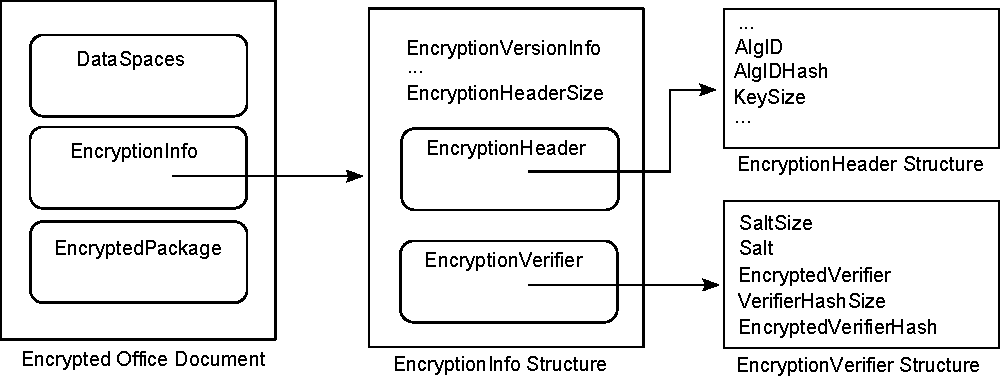
\includegraphics[width=1\textwidth]{figures/ei_struct.pdf}
	\caption{EncryptionInfo structure}
	\label{keys_length}
\end{figure}

Standard encryption describes three algorithms:
\begin{itemize}
	\setlength\itemsep{0.1em}
	\item{key derivation process,}
	\item{verifier generation process and}
	\item{password verification process.}
\end{itemize}

The key derivation process is derived from PKCS \#5: Password-Based Cryptography Version 2.0 as specified in RFC 2898 \cite{rfc2898} and the hashing algorithm used, specified in the \textit{EncryptionHeader.AlgIDHash} field, must be SHA-1. The exact steps to derive the encryption key are as follows:

\begin{enumerate}
\item{Calculate an initial password hash:}
	\begin{itemize}
		\item{$H_0 =\textit{SHA-1(salt + password)}$}
	\end{itemize}
\item{Iterate the hashing using the following approach: 
	\begin{itemize}
		\item{$H_n = \textit{SHA-1(iterator} + H_{n-1})$}
	\end{itemize}
	Variable \textit{iterator} is intially set to 0 and then incremented monotonically until 50,000 iterations have been performed.}
\item{Calculate a final hash:
	\begin{itemize}
		\item{$H_{final} = \textit{SHA-1}(H_n + block)$}
	\end{itemize}
	Variable $block$ is always $0x0000000$.}
\item{The final hash is XORed separately into the first 20-bytes of two buffers containing the bytes $0x36$ and $0x5C$ respectively. The two results of these operations are concatenated and the first $x$ bytes are considered to be the derived key, where $x$ is the key length required by the specified encryption algorithm.}
\end{enumerate}

The key is eventually used to encrypt the given document using AES in ECB mode. ECB is the only supported encryption mode for standard encryption. This implies ECB specific attacks may be applicable. However, the actual encryption process as specified by the EMCA-376 specification needs to be considered. 

When attempting to decrypt the document in order to verify the correctness of a password entered, a password verifier is generated and stored within the \textit{EncryptionInfo} stream. The verifier is 16 bytes long and stored encrypted using AES in ECB mode and a key derived by the aforementioned method. In addition, an encrypted SHA-1 hash of the verifier is also stored. This information is used in the verification process as follows:

\begin{enumerate}
\setlength\itemsep{0.1em}
\item{Derive a key using the aforementioned method from the given user-password.}
\item{Decrypt the value stored in the \textit{EncryptedVerifier} field.}
\item{Decrypt the value stored in the\textit{EncryptedVerifierHash} field.}
\item{Calculate the SHA-1 hash value of the decrypted value calculated in step 2.}
\item{Compare the results of step 3 and step 4. 
	\begin{itemize}
		\item{In case the two values match the password is correct.}
	\end{itemize}}
\end{enumerate}

\begin{figure}[ht]
	\centering
	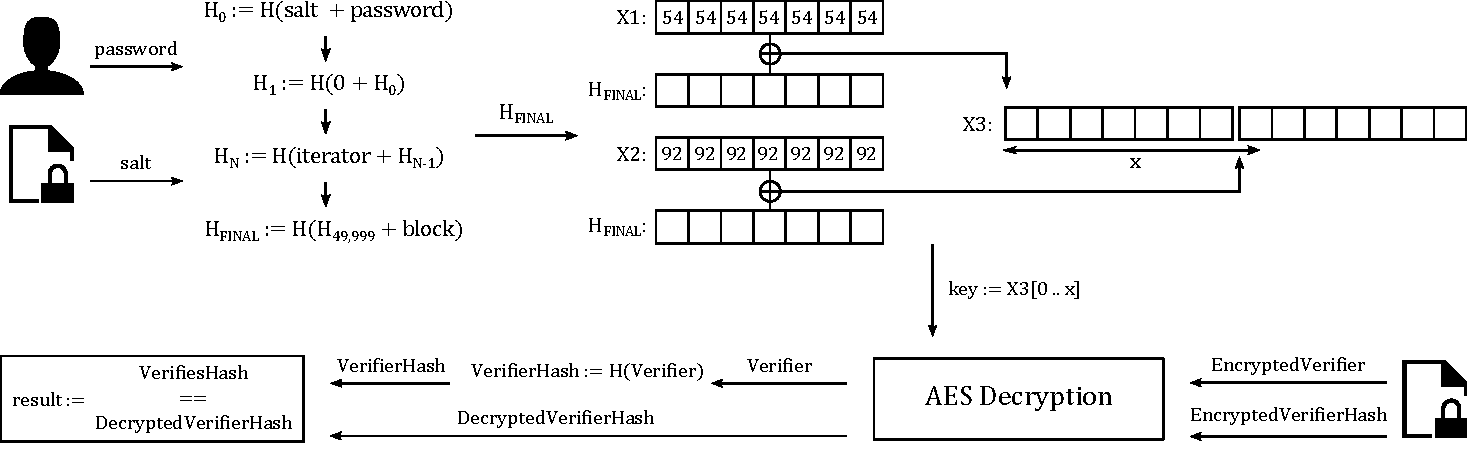
\includegraphics[width=1\textwidth]{figures/standard_encryption_scheme.pdf}
	\caption{Verification process as defined by ECMA-376 standard encryption}
	\label{standard_encryption_scheme}
\end{figure}

\subsection{Agile Encryption}

When agile encryption is used, all information about the cryptography used to encrypt the document is stored in an XML element in the \textit{XmlEncryptionDescriptor} field of the \textit{EncryptionInfo} stream. This element must conform to the XML schema namespace shown in Appendix \ref{ei_agile_stream}. Agile encryption allows a wide range of possible configurations and is therefore much more complex than standard encryption discussed in the previous section. The available algorithms depend on the algorithms that can be accessed through the APIs in the Windows operating system. Microsoft Office 2007 with Service Pack 2 and above support CNG (CryptoAPI: Next Generation). The following listing shows the settings and their default values, which are configurable and change the way files are being encrypted:

\begin{itemize}
\setlength\itemsep{0.1em}
	\item{Set CNG cipher algorithm (default: AES).}
	\item{Configure CNG cipher chaining mode (default: CBC).}
	\item{Set CNG cipher key length (default: 128 bits).}
	\item{Specify encryption compatibility (default: Use next generation format).}
	\item{Set parameters for CNG context (see MSDN \cite{cng_functions}).}	
	\item{Specify CNG hash algorithm (default: SHA1).}
	\item{Set CNG password spin count (default: 100,000).}
	\item{Specify CNG random number generator algorithm (default: RNG).}
	\item{Specify CNG salt length (default: 16 bytes).}
\end{itemize}

A more detailed description of these settings can be found on the Microsoft Developer Network website\footnote{The settings and default values apply to Microsoft Office 2010 and 2013 and are identical.} \cite{plan_office_crypto}. 

Further specified are the steps necessary for deriving keys, generating initialization vectors, and generating a password key encryption structure. This structure is used to verify the correctness of the entered password when trying to open a file and it holds, encrypted, the key used to encrypt the plain-text document. Later in this chapter, this key is referred to as the intermediate key. Appendix \ref{ei_password_encryptor} shows the schema specifying its structure.

For the sake of completeness, it is important to mention that this structure can be represented as a \textit{CertificateKeyEncryptor} structure. The notable difference is that the intermediate key is encrypted using the public part of an X509 certificate instead of a user-supplied password. However, during the research no encrypted document was using this type of key encryptor structure nor was any information found about how to create a document using this type of protection. As a result this approach is not taken into account.

The key derivation process is similar to the method used in standard encryption and also derived from PKCS \#5 \cite{rfc2898}:

\begin{enumerate}
\item{Calculate an initial password hash:}
	\begin{itemize}
		\item{$H_0 =\textit{H(salt + password)}$}
	\end{itemize}
\item{Iterate the hashing using the following approach:}
	\begin{itemize}
		\item{$H_n = \textit{H(iterator} + H_{n-1})$}
	\end{itemize}
\item{Calculate a final hash:}
	\begin{itemize}
		\item{$H_{final} = \textit{H}(H_n + blockKey)$}
	\end{itemize}
\item{If the length of $H_{final}$ is smaller than the key length specified in the \textit{EncryptionInfo}, then the key must be padded by appending bytes with a value of $0x36$. If it is longer, it is truncated to the correct length.}
\end{enumerate}

Note that, unlike in standard encryption, $H()$ is not a fixed hashing algorithm and the $block$ variable depends on the purpose of the key that is being derived. Another difference is that $H_{final}$ is the final key.

Initialization vectors are generated as shown in the following steps:
\begin{enumerate}\label{IVgen}
	\item{If a \textit{blockKey} is provided the IV is:}
	\begin{itemize}
		\item{$H(KeySalt + blockKey)$}
	\end{itemize}
	\item{If a \textit{blockKey} is not provided, then the IV is the \textit{KeySalt}.}
	\item{Depending on the length, the IV is either padded by appending bytes with the value of $0x36$ or truncated to \textit{blockSize} (corresponding to the encryption algorithm specified) bytes.}
\end{enumerate}

\textit{KeySalt} is specified in the document's \textit{EncryptionInfo} and again, the \textit{blockKey} is determined by the IV's purpose.

To understand how the password key encryptor is generated, it is necessary to describe the meaning of some of its elements:

\begin{itemize}
\setlength\itemsep{0.1em}
	\item{\textbf{encryptedVerifierHashInput} -- a random array of bytes encrypted using a key derived from the user-supplied password and a fixed \textit{blockKey}: $0xfe, 0xa7, 0xd2, 0x76, 0x3b, 0x4b, 0x9e, 0x79$.} 
	\item{\textbf{encryptedVerifierHashValue} -- a hash of the plain-bytes of \textit{encryptedVerifierHashInput} encrypted using a key derived from the user-supplied password and a fixed \textit{blockKey}:\\ $0xd7, 0xaa, 0x0f, 0x6d,$ $0x30, 0x61, 0x34, 0x4e$.}
	\item{\textbf{encryptedKeyValue} -- a random array of bytes encrypted using a key derived from the user-supplied password and a fixed \textit{blockKey}: $0x14, 0x6e, 0x0b, 0xe7, 0xab, 0xac, 0xd0, 0xd6$. This element represents the intermediate key.}
\end{itemize}

Note that the intermediate key, used to encrypt the plain-text content of the documents, is randomly generated. Unlike in standard encryption, where the final encryption key was directly derived from the user-supplied password. The specification does not mention anything about how this intermediate key should be generated. In case the key is not generated using a cryptographically secure pseudo-random number generator (CSPRNG), then an implementation specific weakness is introduced and presents a serious flaw in the encryption process. 

In addition to confidentiality, agile encryption also provides a way to verify integrity of encrypted files. Verification is done using the \textit{encryptedHmacKey} and \textit{encryptedHmacValue} attributes of the \textit{EncryptionInfo's DataIntegrity} element. The process of generating this attributes is as follows:

\begin{enumerate}
\setlength\itemsep{0.1em}
	\item{Obtain the intermediate key by decrypting the \textit{encryptedKeyValue} from a \textit{KeyEncryptor structure}.}
	\item{Generate a random array of bytes. This data will be further referred to as \textit{Salt}.}
	\item{Encrypt the \textit{Salt} with the intermediate key. Use an IV generated as specified in \ref{IVgen} with a \textit{blockKey}: \\ $0x5f, 0xb2, 0xad, 0x01, 0x0c, 0xb9, 0xe1, 0xf6$.}
	\item{Result of step 3 becomes the \textit{encryptedHmacKey}.}
	\item{Calculate an HMAC of the entire encrypted document. As a key use the \textit{Salt}.}
	\item{Similarly to step 3. encrypt the result of step 5 using a \textit{blockKey}: $0xa0, 0x67, 0x7f, 0x02, 0xb2, 0x2c, 0x84, 0x33$.}
	\item{Result of step 6 becomes the \textit{encryptedHmacValue}.}
\end{enumerate}

\subsection{Extensible Encryption} 

ECMA-376 documents can optionally utilize user-provided custom encryption modules. As this method is not commonly used it is not further analyzed or discussed.  

\section{Write Protection}

MS Office documents can be protected from unwanted changes. A user is allowed to open and read such files without restrictions. However, any kind of changes is prohibited. A password is required to authenticate the user and disable write protection. The Office Document Cryptography Structure mentions two different protection methods:

\begin{itemize}
\setlength\itemsep{0.1em}
	\item{ECMA-376 Document Write Protection and}
	\item{Binary Document Write Protection.}
\end{itemize}

In general, write protection is not meant to be a security mechanism \cite[p. 94]{msoffcrypto}. The protection can be easily bypassed, no matter which method was used. For this reason only a brief overview of the methods follows.

Write protection for documents represented in a binary format differs by document type:

\begin{itemize}
\setlength\itemsep{0.1em}
	\item{Word and PowerPoint documents -- the password is stored within the document file in plaintext\footnote{PowerPoint documents generated by MS Office PowerPoint 97-2007 Service Pack 1 will encrypt the whole file using the password \textit{/01Hannes Ruescher/01}. Starting with MS Office 2007 SP2 a binary write-protected PPT file will not be encrypted.}. The presence of the password indicates that the client application should enforce write protection.}
	\item{Excel documents -- the password is obfuscated before storing. The document can be encrypted when generated by MS Office Excel 2007 or above. However, this encryption is flawed as a well-known key: \textit{VelvetSweatshop}, is used. This is because the document should be readable for everyone. It helps to prevent direct modifications, i.e. by using a hex editor.}
\end{itemize}

Documents represented in a binary format that are intended to be compatible with ISO/IEC 29500 (Office Open XML File Format) and document files represented as specified in ECMA-376 store the password inside the document file in a hashed form. As an example MS Office Word 2013 will by default calculate the password hash as follows:

\begin{enumerate}
\item{Calculate an initial password hash:}
	\begin{itemize}
		\item{$H_0 =\textit{SHA1(salt + password)}$}
	\end{itemize}
	The salt is generated using an arbitrary pseudorandom function.
\item{Iterate the hashing 100,000 times using the following approach:}
	\begin{itemize}
		\item{$H_n = \textit{SHA1(iterator}+ H_{n-1})$}
	\end{itemize}
	Iterator is represented as a 32-bit integer initially set to 0.
\item{$H_{99,999}$ becomes the resulting hash.}
\end{enumerate}

Note that the iteration count and hashing function are configurable. This approach helps to protect the user-specified password when the document itself gets leaked to unauthorized users. However, removing the whole hash entry from the file will effectively remove the write protection.

\section{Digital Signatures}\label{data_integrity}

Similarly to write protection and encryption, digital signatures are different between binary Office documents and Office documents represented as specified in ECMA-376. There are two digital signature formats:

\begin{itemize}
\setlength\itemsep{0.1em}
	\item{CryptoAPI Digital Signature}
	\item{Xmldsig Digital Signature}
\end{itemize}

Both are applicable for binary documents. ECMA-376 documents use the Xmldsig Digital Signature. Digital signatures are used to detect changes. They do not prevent users from making modifications to the document. However, MS Office applications will not allow any changes until valid signatures are not explicitly removed.

\subsection{CryptoAPI Digital Signature} 

A digitally signed binary document must contain a stream named \textit{\_signatures}. This stream contains at least one signature and the corresponding certificate. Only X.509 certificates using RSA as the signing algorithm are allowed. They need to be stored in ASN.1 DER encoding. It also contains a timestamp which specifies when the signature was created. The document parts which shall be signed must be hashed using the MD5 function. Using the MD5 hash function introduces possibilities for collision attacks and practical attacks may be realistic, similarly to attacks demonstrated on PKI \cite{md5_vulnerable}. 


\subsection{Xmldsig Digital Signature}

Xmldsig Digital Signatures are stored as a stream in the \textit{\_xmlsignatures} folder. Every document can have one or more signatures. Signatures are stored separately. A single signature is represented as specified by W3C in XML Signature Syntax and Processing \cite{xmlsig}. XML Advanced Electronic Signatures \cite{xades} extensions are also allowed.

Xmldsig digital signatures are used in Office 2007 and above by default. This is true for both binary documents and ECMA-376 documents. In Office 2007 signed document parts are hashed using SHA-1. Note that it is the only supported hash algorithm. Higher versions can use any hash algorithm that is supported by the underlying operating system. As an example Office 2013 uses SHA-256.

\section{Summary}

The structure of MS Office documents is very complex and changed heavily over time. Major differences can be seen between documents represented as specified by ECMA-376 and binary representation. ECMA-376 encryption methods are evolving over time, to reflect current trends and provide protection from modern threats. For example the default encryption mode changed from ECB to CBC and a whole new element providing data integrity was introduced. Binary protection methods, such as XOR obfuscation or 40-bit RC4 encryption, are out dated and do not provide sufficient level of security. However, this is clearly stated directly by the specification \cite[p. 93]{msoffcrypto}. Similarly, when using agile encryption or extensible encryption, use of modern hashing and encryption algorithms is explicitly recommended.

Passwords used for write protection are strongly protected. This is very important as people are used to reuse passwords commonly. Storing any kind of user-defined passwords inside the document structure in hashed form is definitely reasonable and correct. Of course, the hashing process should be intentionally slow to stop determined attackers. Write protection itself is not considered to be a security mechanism. It can be always bypassed. 

Digital signatures provide confirmation that the document's content originated from the signer and has not been altered with. Implementation of digital signatures is straightforward and based on common standards XML Signature Syntax and Processing \cite{xmlsig} and XML Advanced Electronic Signatures \cite{xades}. 

Microsoft Office is implementing all mentioned protections using modern cryptographic algorithms with strong defaults. 

\chapter{Portable Document Format}

Document protections of the Portable Document Format (PDF) files will be discussed in details necessary in context of this thesis. All information is based on two publicly available specifications:

\begin{itemize}
\setlength\itemsep{0.1em}
\item{Adobe® Supplement to the ISO 32000 \cite{iso32000sup} and}
\item{Document management — Portable document format — Part 1: PDF 1.7 \cite{pdf_spec}.}
\end{itemize}

The focus is on differences between various versions and how the protections evolved over time. As the file structure of PDF files is rather complicated and extensive the focus is, for the sake of simplicity, on parts specifically relevant to protection mechanisms.

\section{Encryption}

The encryption mechanism was introduced in PDF version 1.1. All encryption related information is stored in the document's trailer dictionary \cite[p. 42]{pdf_spec} within an encryption dictionary. The presence of the encryption dictionary implies that the document is encrypted.

Every encryption dictionary is required to specify the name of the preferred security handler for the document. The handler is a software module that implements aspects of the encryption process and controls access to the contents of an encrypted document. A standard password-based security handler and a public-key security handler are defined directly by the PDF specification. All algorithms discussed further in this chapter are specific for these standard security handlers.

\subsection{Standard Security Handler}\label{pdf_enc}

Unlike other formats discussed (MS Office, Open Document Format) PDF's standard security handler allows the user to define access permissions and two passwords: an owner password and a user password. The user password is enough to decrypt a document. The owner password is needed in case the user wants to modify the access permissions of the document.

Table \ref{handler_entries} shows encryption dictionary entries defined by the standard security handler which are important in the algorithms described later in this chapter.

\begin{table}[hp]
	\centering
	\begin{tabular}{|l|l|}
               	\hline
		\textbf{Key}&\textbf{Value}\\
		\hline
		V&Specifies the algorithm used to encrypt \\
		&and decrypt the document.\\
		&\textbf{0} -- An algorithm that is undocumented.\\
	`	&This value shall not be used.\\
		&\textbf{1} -- RC4 or AES with a key of length 40 bits.\\
		&\textbf{2} -- RC4 or AES permitting keys longer then 40 bits.\\
		&Available since PDF 1.4.\\
		&\textbf{3} -- An unpublished algorithm permitting keys\\
		&of lengths from 40 to 128 bits.\\
		&This value shall not be used in conforming PDF files.\\
		&\textbf{4} -- A more sophisticated encryption and decryption\\
		&process using rules defined in additional entries\\
		&of the dictionary. Available since PDF 1.5.\\
		&\textbf{5} -- Same as 4 but allows the use of keys with length\\
		&256 bits.\\
	\hline
		R&Specifies the revision of the security handler.\\
		&Can have values from 2 to 5 and mostly depends on V.\\
	\hline
		O&A 32-byte (for R being 1-4) or 48-byte (for R being 5)\\ 
		&string based on both the owner and the user password.\\
		&Used in the owner password verification process.\\
	\hline
		U&A 32-byte (for R being 1-4) or 48-byte (for R being 5)\\ 
		&string based on the user password.\\
		&Used in the user or owner password verification process.\\
	\hline
		P&A set of flags representing access permissions.\\
	\hline
		EncryptMetadata& In case V is of value 4 (PDF 1.5) indicates\\
		&if document metadata should be encrypted.\\
	\hline
           \end{tabular}
	\caption{Encryption dictionary entries defined by the standard security handler \cite{pdf_spec}}
	\label{handler_entries}
\end{table}

The owner-based or user-based encryption keys are computed using the following algorithm by standard security handlers of revision 1-4: 

\begin{enumerate}
\setlength\itemsep{0.1em}
\item{If the password is longer than 32 bytes\footnote{The password is represented in PDFDocEncoding \cite[157]{pdf_spec}. 32 bytes can represent 32 characters.} use only its first 32 bytes. Otherwise, pad it by appending bytes from the beginning of the following default 32-byte padding string: $28$ $BF$ $4E$ $5E$ $4E$ $75$ $8A$ $41$ $64$ $00$ $4E$ $56$ $FF$ $FA$ $01$ $08$ $2E$ $2E$ $00$ $B6$ $D0$ $68$ $3E$ $80$ $2F$ $0C$ $A9$ $FE$ $64$ $53$ $69$ $7A$. In case no user-password is provided, the whole padding string is used.}
\item{Using a MD5 hash function compute a hash of the following data:}
	\begin{itemize}
		\item{The result of step 1.}
		\item{The encryption dictionary's O entry.}
		\item{The encryption dictionary's P entry.}
		\item{The first element of the file's identifier array \cite[p. 43]{pdf_spec}.}
		\item{4 bytes with the value $0xFFFFFFFF$ if document metadata is not being encrypted.}
	\end{itemize}
\item{For revision 3 or greater hash the first $n$ bytes of the output using MD5, where $n$ is the length of the required encryption key as defined in the encryption dictionary. Repeat this step 50 times.}
\item{The first $n$ bytes become the computed encryption key.}
\end{enumerate}

The O entry is basically the user password encrypted by a owner-password-based key. The algorithm is as follows:

\begin{enumerate}
\setlength\itemsep{0.1em}
\item{Pad or truncate the owner password the same way as described in the previous algorithm.}
\item{Hash the output of step 1 using the MD5 hash function.}
\item{For revision 3 or greater hash the output of previous step using the MD5 hash function. Repeat this step 50 times.}
\item{Use the first $n$ bytes as an RC4 encryption key, where $n$ is 5 for handlers of revision 2. For handlers of revision 3 or greater $n$ is the length of the encryption key as defined in the encryption dictionary.}
\item{Pad or truncate the user password the same way as described in the previous algorithm and encrypt it using RC4 with the key obtained in the previous step.}
\item{For revision 3 or greater repeat the following 19 times: Take the output of the previous invocation of RC4 and pass it as input to a new invocation. The encryption key for every iteration is created by performing an XOR operation between each byte of the encryption key obtained in step 4 and the byte value of the iteration counter (values 1-19).}
\end{enumerate}

The U entry is for handlers of revision 2 the default 32-byte padding string encrypted using the user-password-based encryption key. For handlers of revision greater than 3 the way how the U entry is calculated changed. The algorithm is as follows:

\begin{enumerate}
\setlength\itemsep{0.1em}
\item{Using a MD5 hash function compute a hash of the following data:}
\begin{itemize}
		\item{the default 32-byte padding string, and}
		\item{the first element of the file's identifier array \cite[p. 43]{pdf_spec}.}
\end{itemize}
\item{Encrypt the result using RC4 with the user-password-based encryption key.}
\item{Do the following 19 times: Take the output of the previous invocation of RC4 and pass it as input to a new invocation. The encryption key for each iteration is created by performing an XOR operation between each byte of the encryption key obtained in step 4 and the byte value of the iteration counter (values 1-19).}
\item{Append 16 bytes of arbitrary padding to the output of the previous step.}
\end{enumerate}

Note that the user-password-based encryption key is used to decrypt contents of the document. The owner-password-based key is used to verify correctness of the provided owner-password.

In revision 5 all algorithms previously mentioned were completely replaced. Two new encryption dictionary entries were introduced (see table \ref{additional_handler_entries}). 

\begin{table}[h]
	\centering
	\begin{tabular}{|l|l|}
               \hline
		\textbf{Key}&\textbf{Value}\\
	\hline
		OE&A 32-byte string based on the owner and user passwords.\\
		UE&A 32-byte string based on the user password\\
	\hline
           \end{tabular}
	\caption{Encryption dictionary entries introduced by standard security handlers of revision 5}
	\label{additional_handler_entries}
\end{table}

The maximum password length was extended from 32 bytes to 127 bytes. As mentioned before the U and O entries were extended to 48 bytes and represent 3 logical parts. The first 32 bytes are a verification hash. The next 8 bytes are a validation salt. The last 8 bytes are a key salt. The OE and UE values contain the file encryption key encrypted by an owner-password-based or user-password-based key, respectively.

At this point the publicly available supplement to the ISO 32000 \cite{iso32000sup} appears to be incomplete in terms of the file's encryption key computation. A new \textit{Computing an encryption key} algorithm is described. This algorithm includes a step where decrypting the OE, or UE, value is necessary to get the file encryption key. Algorithms to generate the OE and UE values include a step where encrypting the file encryption key is necessary. However, the origin of the file encryption key is not mentioned. 

The process of password verification is straightforward:

\begin{enumerate}
\setlength\itemsep{0.1em}
\item{Truncate the provided password to 127 bytes\footnote{The password is based on Unicode (UTF-8 encoding).} if it is longer than 127 bytes.}
\item{Compute the SHA-256 hash of the password concatenated with 8 bytes of the owner validation salt and the 48-byte U value.}
\item{In case the result matches the 32-byte verification hash of the O value, the provided password is the correct owner password.}
\item{Compute the SHA-256 hash of the password concatenated with 8 bytes of the user validation salt.}
\item{In case the result matches the 32-byte verification hash of the U value, the provided password is the correct user password.}
\end{enumerate}

An interesting observation can be seen after describing the way of verifying a password provided by the user. The only computation that has to be done to verify a given password is calculating one SHA-256 hash value. This approach actually weakens the strength of the document protection as discussed in more detail in section \ref{pdf_summ}.

Algorithms mentioned up to this point, are all publicly available and documented directly by Adobe. However, PDF files using a standard security handler of revision 6 are generated when using Adobe Acrobat Pro X or higher. A quick look at the preview of \textit{ISO/DIS 32000-2.4 Document management -- Portable document format -- Part 2: PDF 2.0} reveals that indeed standard security handlers of revision 6 and higher are mentioned. However, it is possible to find the actual key verification algorithm publicly on the Internet \cite{esec_lab}. The algorithm is similar to the algorithm used by security handlers of revision 5. It adds a minimum of 32 rounds of obscure AES-128 encryption followed by SHA-2 hashing.

\subsection{Public-Key Security Handlers}

In addition to password-based encryption, security handlers may use asymmetric encryption. Instead of specifying a password, it is necessary to specify one or more  lists of recipients. Every such list can have different access permissions specified. 

When encrypting a document using a public-key security handler, each recipient's X.509 public certificate part must be available. When opening such a protected document, the recipient has to provide the corresponding private key.

A public-key encryption dictionary is mostly similar to a password-based encryption dictionary. It contains one extra field named \textit{Recipients}. It represents an array of lists of recipients. Within one list all recipients have the same access permissions. 

Figure \ref{public_key_alg} illustrates the process of decrypting a protected PDF file using a standard public-key security handler.

\begin{figure}[ht]
	\centering
	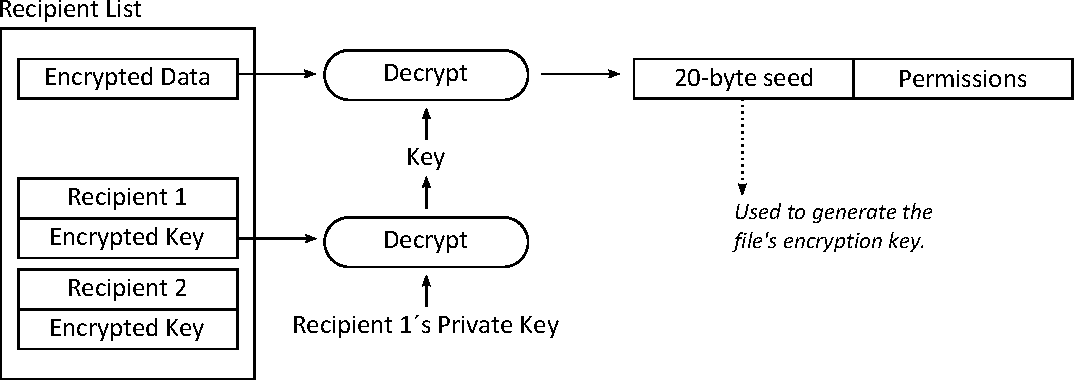
\includegraphics[width=1\textwidth]{figures/public_key_alg.pdf}
	\caption{Decryption process when using standard public-key security handlers. Based on \cite[p. 130]{pdf_spec}}
	\label{public_key_alg}
\end{figure}

Every recipient list contains a 20-byte seed, which is used to generate the file's encryption key, and a 4-byte value specifying access permissions. The seed should be, according to the specification, a unique random number generated by the security handler. Both the seed and the permissions value are stored within the list in an encrypted manner. The encryption algorithm can be any of the following: 


\begin{itemize}
\setlength\itemsep{0.1em}
	\item{RC2 with key lengths up to 128 bits,}
	\item{RC4 with key length up to 256 bits,}
	\item{DES, Triple DES,}
	\item{AES-128-CBC, AES-256-CBC or AES-192-CBC.}
\end{itemize}

Adobe's Acrobat products use Triple DES by default (all mentioned are supported when decrypting documents). Note that no comments or requirements are given about key generation. Implementation mistakes may lead to a serious vulnerability, if this key is not generated using a CSPRNG. The attacker could learn the value of the seed without actually having a corresponding private key. The key is stored inside the recipient list, encrypted using the recipient's public key. 

Once the seed is known, the file's encryption key can be computed as follows:

\begin{enumerate}
\setlength\itemsep{0.1em}
	\item{Compute the SHA-1 hash of the 20-byte seed concatenated with the whole value of the \textit{Recipients} field and 4 bytes with the value $0xFF$ if document metadata is not encrypted.}
	\item{The first $n$ bytes of the resulting hash become the encryption key, where $n$ is determined by other fields of the encryption dictionary.}
\end{enumerate}

The above algorithm implies that the length is upper-bounded by the output length of the SHA-1 hashing function -- 20 bytes. The specification indicates that the document will be always encrypted using the RC4 cipher, which makes sense as the key length is limited to 128 bites (16 bytes). This leads to the assumption that a custom public-key security handler is needed to change this behavior.   

\section{Digital Signatures}
Digital signatures are supported in PDF 1.3 and higher versions. Processing of signatures is implemented by a plug-in signature handler. The PDF specification is explicitly encouraging third-party handler writers to register their handlers with Adobe \cite[p. 725]{pdf_spec}.

The common way to create signatures is to compute a digest of the document (or some part of the document) and store the digest within the same document. To verify a signature the user has to repeat the same process and compare the results. All signature information is stored within a signature dictionary.

Two techniques to compute such digests are defined:

\begin{itemize}
\setlength\itemsep{0.1em}
	\item{Computing a \textit{byte range digest} -- the \textit{ByteRange} field of the signature dictionary indicates a range of bytes over which the digest is computed. Typically the range is the entire file.}
	\item{Computing a \textit{object digest} -- the digest is computed by selectively going through the document's objects, typically beginning with the root object. The exact way to compute the digest is described within the \textit{TransformMethod} and \textit{TransformParams} fields of signature reference dictionary. This technique is available since PDF 1.5.}
\end{itemize}

Moreover, different types of signatures are defined. The specification mentions \textit{ordinary} signatures, MDP (modification detection and prevention) signatures, usage rights signatures and signatures of FDF files. A brief overview follows:

\begin{itemize}
\setlength\itemsep{0.1em}
	\item{\textit{Ordinary signatures} -- computed as a byte range digest described above. It represents a typical signature as known in other document formats.}
	\item{\textit{MDP signatures} -- enables the author of the document to define what changes are permitted to be made on the signed document, and what changes will invalidate the current signature.}
	\item{\textit{User rights signatures} -- allows to enable interactive document-based features that are not available in some client applications (e.g. Adobe Reader) by default.}
	\item{\textit{FDF file signatures} -- a special signature type used in Forms Data Format (FDF) files \cite[p. 710]{pdf_spec}.}
\end{itemize}

Note that the specification covers the features of each type in very detail. It also specifies interoperability between various signature types, revocation methods and permission handling (similar to access permission discussed in subsection \ref{pdf_enc}, but without the necessity to encrypt the file). PDF's signature features include very complex functionality \cite{acrobat_dig_signatures} and covering them all exceeds the scope of this thesis. An overview of particularly interesting features follows:

\begin{itemize}
\setlength\itemsep{0.1em}
	\item{\textbf{Alternative signature methodologies} -- in addition to digital signatures leveraging asymmetric cryptography, biometric forms of identification, such as fingerprints, handwritten signatures or retinal scans, can be used.}
	\item{\textbf{Robust algorithm support} -- strong encryption algorithms, like RSA with keys of length up to 4096 bits and hash functions SHA-512 or RIPEMD160 are all supported by signature handlers created by Adobe.}
	\item{\textbf{Incremental updates} -- changing digitally signed documents, without invalidating the current signatures, is possible. All modifications can be later detected and audited.}
\end{itemize}

\section{Summary}\label{pdf_summ}

Password-based encryption done by standard security handlers is rather questionable. A shift from older insecure cryptographic algorithms, like RC4 and MD5, is a step in the right direction. However, the replacement introduced in security handlers of version 4 revision 5 rendered the protection level less secure, in terms of offline brute-force capabilities. As one iteration of SHA-256 hashing reveals the correctness of a given password, it is extremely easy to lunch effective offline attacks. Latest security handlers introduced a more sophisticated way of password derivation leveraging AES encryption. There seems to be no obvious reason not to use common password derivation functions like PBKDF2, which provide comparable benefits even with a low iteration count (see figure \ref{average_speed}). 

A better solution is to use public-key security handlers if offline brute-force attacks are considered a threat. However, this means that the document will be encrypted using RC4, which may lead to attacks leveraging known vulnerabilities in RC4. 

Portable Document Format provides very advanced and extensible mechanism for digital signatures. Support for alternative signature methodologies, incremental updates and robust algorithm support, render it superior compared to other discussed document formats. Adobe also explicitly encourages third parties to register new signature handlers. A further detailed review on digital signatures in PDF and existing implementations of signature handlers may be very educative and useful.  

\chapter{Open Document Format for Office Applications}

Documents in the Open Document Format can be represented in two ways \cite{odt_spec}:

\begin{itemize}
\setlength\itemsep{0.1em}
\item{A single XML document.}
\item{A collection of files within a package, each of which stores a portion of the document.}
\end{itemize}

Particularly important in the context of this paper is the second method. All protection mechanisms defined apply to packages. A package representing a single Open Document Format file will be referred to as \textit{ODT package} from this point forward.

\section{Encryption}\label{odt_enc}

The encryption process as specified in Open Document Format for Office Applications (\textit{OpenDocument}) \cite{odt_spec} has 3 stages:

\begin{enumerate}
\setlength\itemsep{0.1em}
	\item{The user-supplied password is hashed.}
	\item{For each file to be encrypted, a separate key is generated using the hashed password and the PBKDF2 algorithm \cite{rfc2898}.}
	\item{The files are encrypted using the keys created in step 2.}
\end{enumerate}

The exact algorithms and other necessary cryptographic parameters are defined in the document's manifest. The manifest is a mandatory part of every ODT package and its relative path within the package must be \texttt{META-INF/}
\texttt{manifest.xml}. The manifest is an XML file conforming to the XML schema shown in Appendix B.

For every file in the ODT package the manifest must contain an element denoted as \texttt{<manifest:file-entry>}.

\begin{figure}[ht]
	\centering
	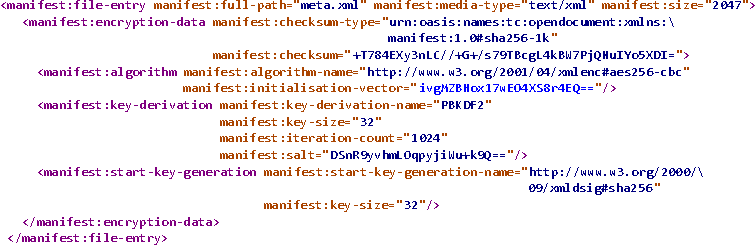
\includegraphics[width=1\textwidth]{figures/manifest_snippet.pdf}
	\caption{Example of a file entry element within an ODT document's manifest file}
	\label{manifest_snippet}
\end{figure}

A \texttt{<manifest:encryption-data>} child element indicates that the file is stored encrypted within the package. It also contains information required to decrypt the particular file. The attribute \texttt{manifest:checksum-type} specifies a digest algorithm used to calculate a hash of the file. This hash is stored in the \texttt{manifest:checksum} attribute in BASE64 encoding. 
The algorithm used to encrypt a file is specified in the \texttt{manifest:algorithm-name} attribute of the \texttt{<manifest:algorithm>} element. If the algorithm requires an initialization vector, then it is specified in the \texttt{manifest:initialization-vector} attribute.
In a similar fashion, the elements \texttt{<manifest:key-derivation>} and \texttt{<manifest:start-key generation>} specify how the start key is generated from the user password and how the encryption key is derived from the start key, respectively.
All algorithms that can be used for the purposes discussed in this section, and which should be supported by implementations, are listed in the Open Document Format specification. New algorithms were added as the specification was extended over time. 

Versions 1.0 and 1.1 specified SHA-1 as the only hash function for the \texttt{manifest:checksum-type} and \texttt{manifest:start-key-generation-name} attributes. The only available \texttt{manifest:algorithm-name} was Blowfish in CFB mode. Version 1.2 introduced support for additional hash functions and algorithms: SHA-256, SHA-512, RIPEMD-160, 3DES, AES-128, AES-256, and AES-192. The only available key generation algorithm in all three versions is PBKDF2.

\section{Digital Signatures}

Digital signatures have been defined ever since version 1.2. One package may contain multiple signatures. All signatures are located within the \texttt{META-INF/} folder and should contain the term \textit{signature} in their name. Every signature has to explicitly list all files that are being validated. In particular, all files should be referenced by some signature to ensure the integrity of the entire document.

The Open Document Format specification describes that digital signature can be used together with encrypted packages in two ways. The signature can be applied to encrypted files and should be validated prior to decrypting the package. The other option is digitally signing the package before encrypting it. This approach will also encrypt the files containing digital signatures.  

However, popular implementations seem to only support the first-mentioned approach. Once a digitally signed file is encrypted, all signatures are removed before encrypting the file. The file has to be manually re-signed again.

\section{Summary}

Protections described in the Open Document Format are rather simple and clearly described. Focus on security can be seen when looking at differences of various versions. Version 1.2 introduced a mechanism for digital signatures as well as support for modern cryptographic functions. The use of PBKDF2 with configurable iteration count allows for the mitigation of simple offline brute-force attacks. However, GPU powered attacks may become extremely successful as PBKDF2 is not designed to be memory-hard \cite{PBKDF2_attack}.

Two popular implementations have been tested: LibreOffice and Apache OpenOffice. Both applications were used in the latest stable version released at the time - for LibreOffice this was version 5.2.2 and for OpenOffice version 4.1.3. An overview of the results is shown in table \ref{odt_impl_results}.

\begin{table}[h]
	\centering
	\begin{tabular}{|l|l|l|}
               \hline
		&\textbf{LibreOffice}&\textbf{Apache OpenOffice}\\
	\hline
		manifest:checksum-type&SHA-256&SHA-1\\
	\hline
		manifest:algorithm-name&AES-256&Blowfish CFB\\
	\hline
		manifest:start-key-derivation-name&SHA-256&SHA-1\\
		manifest:key-derivation-name&PBKDF2&PBKDF2\\
		manifest:iteration-count&1024&1024\\
		manifest:key-size&32&16\\
	\hline
           \end{tabular}
	\caption{Comparsion of document protections methods used by LibreOffice and Apache OpenOffice}
	\label{odt_impl_results}
\end{table}

Both applications encrypt all files in the package. Similarly, both applications include all files when applying a digital signature to the document. A particularly interesting finding is that Open Office prefers the Blowfish algorithm for encrypting documents.

\chapter{Distributed Password Recovery}

As people tend to forget passwords, it is likely that access to password-protected documents can be lost. A straightforward solution in this case is brute-force, as password verification is done offline. To show and further discuss the speed and efficiency of this process, a distributed password recovery system was created.

The implementation and any files mentioned in this chapter can be found on the attached CD or in the official thesis archive available at \textit{http://is.muni.cz/}.

\section{System Overview}

The whole system consists of 3 logically separated parts depicted in figure \ref{ddpbf_design}. 

\begin{figure}[ht]
	\centering
	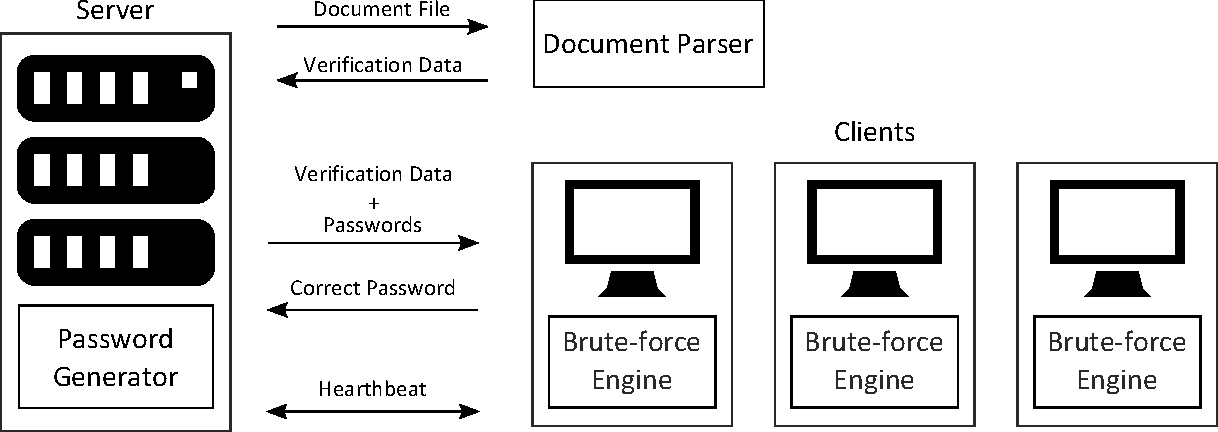
\includegraphics[width=1\textwidth]{figures/ddpbf_design.pdf}
	\caption{Distributed password recovery design}
	\label{ddpbf_design}
\end{figure}

The input for the system is a password protected Office, PDF or ODT document. As the password verification process can be very different among these formats, a detailed list of currently supported algorithms follows:

\begin{itemize}
\setlength\itemsep{0.1em}
	\item{MS Office Document Structure -- Standard Encryption (as described in subsection \ref{msoff_standard_enc}).}
	\item{Portable Document Format --  version 1.3 to 1.7 using standard security handlers from version 1 to 5 and revision 2 to 6 (as described in subsection \ref{pdf_enc}).}
	\item{Open Document Format – version 1.2 using AES-256 (as described in subsection \ref{odt_enc}).}
\end{itemize}

The basic idea is that the server part acts as the main entry point for the user and handles all additional work. It utilizes a document parser to gather information necessary for password verification and distributes work among all active clients. A more detailed description of every part follows. 

\subsection{Client-server model}\label{client-server}

The server provides a simple command line interface and can be started using the following command: 

\begin{lstlisting}
$ python server.py [-h] [-pr PASSWORDRANGE] [-ps PAYLOADSIZE] document_type filename tcp_ip tcp_port
\end{lstlisting}

Note that the current version must be run with Python 2.7 in order to function properly. A detailed description of the arguments follows:

\begin{itemize}
\setlength\itemsep{0.1em}
	\item{\textbf{-h} -- Shows a descriptive help message.}
	\item{\textbf{-pr} -- Sets the password's maximum length (default: 8).}
		\begin{itemize}
		\setlength\itemsep{0.1em}
			\item{All passwords up to the specified length will be checked.}
		\end{itemize}
	\item{\textbf{-ps} -- Number of passwords sent to each client on every connection (default: 20,000).}
	\item{\textbf{document\_type} -- Number identifying the given document's type.}
		\begin{itemize}
		\setlength\itemsep{0.1em}
			\item{1 -- Microsoft Office}
			\item{2 -- Open Document Format}
			\item{3 -- Portable Document Format}
		\end{itemize}
	\item{\textbf{filename} -- Path to the document file which's password should be recovered.}
	\item{\textbf{tcp\_ip, tcp\_port} --  IP address and port number to which clients should connect in order to communicate with the server.}
\end{itemize}\label{server_params}

When run, the server extracts all information necessary to perform the password recovery process. This is accomplished by calling one of the document parsers described in subsection \ref{doc_parsers}. Afterwards the server passively waits for clients to connect. Once connected, the server sends the verification data and a list of passwords in JSON \cite{rfc7159} format:

\begin{lstlisting} 
{"passwords":[<passwords>], "data":"<document_parser_output>"}
\end{lstlisting}\label{server_message}

Passwords are generated in a separate sub-process and placed into a synchronized queue. To prevent massive memory consumption, the number of items in the queue must never exceed the limit of 2 times the password chunk size that is sent to clients (set by the \textit{–pr} argument).

A list of active clients is maintained by the server. Every client is clearly identified by a universally unique identifier (UUID) \cite{rfc4122}. When setting the \textit{–pr} argument to a high value, the time interval between two messages exchanged between a client and the server might be very high (even days). This is because the client will ask for a new list of passwords after it successfully verifies all the passwords it has received. To recognize inactive clients (e.g., the client machine was terminated, etc.) a heart beat mechanism is implemented. Every 20 seconds, a small message (heart beat) is sent to the server. As a result, any client not connecting to the server for longer than 120 seconds will be marked as inactive. In the event a client connects at any later point, it will be treated as a new client. There is no maximum number of clients, which allows theoretically for an unlimited linear growth in performance. The server keeps track of what passwords were sent to which client. This prevents losing passwords in case a client becomes unresponsive. Once a client is marked inactive, all passwords that were currently processed by it are eventually resent to another client. 

On every client connection (excluding heart beats) an update is logged. This update contains the current number of active clients and an estimate of the current recovery speed. Every password has to go through a hashing process to be verified. Therefore, the speed is represented by the number of tried passwords per second. The speed is naïvely computed as the ratio of the elapsed time and passwords processed by clients. This implies that the server cannot estimate a speed before at least one client asks repeatedly for more passwords. The server will automatically shut down when it receives the correct password from a client.

The client can be run using the following command:
\begin{lstlisting}
$ python client.py [-h] tcp_ip tcp_port 
\end{lstlisting}

The \textit{tcp\_ip} and \textit{tcp\_port} are the connection parameters used to communicate with the server. The optional \textit{–h} argument will show a descriptive help message. 

Once run, the client generates a UUID and immediately sends a message to the server asking for a password list and any verification data. This information is then passed to the brute-force engine described in subsection \ref{brute_force_engine}. The actual brute-forcing is separated from the client on purpose. The reason for this is to keep the system as modular as possible. It is important to note that this approach allows any brute-force engine to be used (e.g., hashcat or JtR \cite{hashcat, jtr} described in more detail in section \ref{related_work}).\label{jtrhc_modular} Once complete, the result is sent to the server. In the event the password was not found, the client will receive a new password list and repeat the whole process.

\subsection{Document parsers} \label{doc_parsers}

The document parsers are stand-alone Python scripts that take document files as input and return all  data necessary for the verification process. Note that the scripts used to extract information from PDF and MS Office files were not created as part of this thesis, but rather taken from the public \textit{John the Ripper} GitHub repository.\footnote{Available at \textit{https://github.com/magnumripper/JohnTheRipper}} Small modifications were made to these scripts, to better fit into the developed system. All changes are included as comments in the respective files. Parsing of ODT files was implemented as part of this thesis. The parser accepts as valid input, ODT files conforming to the latest specifications (version 1.2).

\subsection{Brute-force engine}\label{brute_force_engine}

The brute-force engine can be used either as a stand-alone Python script providing a simple command line interface, or as a Python module. When run separately, it can be started using the following command:

\begin{lstlisting}
$ python brute_force.py [-h] [-pr PASSWORDRANGE] document_type filename
\end{lstlisting}

All the parameters correspond to the identically named parameters described in subsection \ref{server_params}. Once the engine is invoked this way, it parses the given document and initializes a password range based brute-force process. Passwords are generated and placed in a synchronized queue in a separate process. The passwords in the queue are being pulled one by one and verified using a \textit{password verifier}. There are 3 separate verifiers for the supported documents, respectively. All three verifiers are written in plain C and the script utilizes Python's multiprocessing module to invoke more instances simultaneously. C was chosen for performance reasons, as it was shown that a plain rewrite from Python to C sped up the verification process by approximately 4 times. The code snippet below shows the methods responsible for calling these verifiers.

\begin{lstlisting}
def _call_msoffcrypto_core(pwd, input_data):
    return Popen(["ms-offcrypto-impl/./msoffcrypto", pwd, 
        input_data[5], # salt
        input_data[4], # salt_length
        input_data[6], # encrypted_verifier
        str(len(input_data[6]) / 2), # enc_verifier_length
        input_data[7], # encrypted_verifier_hash
        str(len(input_data[7]) / 2), # enc_verifier_hash_length
        str(input_data[3]), # aes_key_length
        str(input_data[2]), # verifier_hash_size
        ])

def _call_odt_core(pwd, input_data):
    return Popen(["odt-impl/./odt", pwd, 
        input_data[2], # checksum
        input_data[3], # iv
        input_data[4], # salt
        input_data[5], # encrypted_file
        str(input_data[6]), # encrypted_file_length
        ]) 

def _call_pdf_core(pwd, input_data):
    return Popen(["pdf-impl/./pdf", pwd, 
        input_data[1], # version
        input_data[2], # revision
        input_data[3], # length
        input_data[4], # p
        input_data[5], # meta_encrypted 
        input_data[6], # id_length 
        str(input_data[7]), # id
        input_data[8], # u_length 
        str(input_data[9]), # u 
        input_data[10], # o_length
        str(input_data[11]) # o
        ]) 
\end{lstlisting}


In a similar fashion these verifiers can be called directly and accept a \textit{–v} argument to enable verbose output for debugging purposes. Note that the verifiers use the OpenSSL library for C \cite{openssl} to perform all cryptographic operations. Therefore, when compiling them, it is necessary to add a link to the library (i.e., using \textit{-lssl} and \textit{-lcrypto} switches when compiling with \textit{GCC}).

Additionally, the script provides a public \textit{init()} method that, requires either a password range or a list of passwords as an argument. If a password range is given, then the script generates its own list. This is done using a naïve generator, which generates all possible variations of words consisting of lower case letters up to the given range. As an example, if the specified range is 2, then the resulting generated word list contains the characters \textit{a} to \textit{z} and words \textit{aa} to \textit{zz}. Otherwise, the provided list of passwords is directly placed into a synchronized processing queue. The second approach is used in the client-server model discussed in subsection \ref{client-server}. It is important to note that this allows the engine to be easily modified to use a wordlist as input. A wordlist approach can, in general, be more efficient than plain brute-forcing of passwords, which can in turn result in a faster password recovery.

\section{Related Work}\label{related_work}

\section{Testing and Results}

The distributed password recovery framework was deployed in a virtualized environment. The environment was provided by the Centre for Research on Cryptography and Security (CRoCS). The setup consisted of 4 machines. One machine was used as the control server, the remaining three were clients. All were part of one local subnet. Every machine had 4 virtualized CPUs and 2 GB of RAM available. 

The objective was to evaluate the capability of withstanding offline brute-force attacks. The following document types were tested:

\begin{itemize}
\setlength\itemsep{0.1em}
	\item{Microsoft Word 2007 -- uses standard encryption as described in subsection \ref{msoff_standard_enc}.}
	\item{LibreOffice Writer 5.2.2 -- uses protections as described in section \ref{odt_enc}.}
	\item{PDF 1.3 with a standard security handler of version 1 revision 2.}
	\item{PDF 1.7 with a standard security handler of version 4 revision 4.}	
	\item{PDF 1.7 with a standard security handler of version 4 revision 5.}	
	\item{PDF 1.7 with a standard security handler of version 4 revision 6.}	
\end{itemize}

Note that the PDF variants were chosen to highlight differences between various protection mechanism. These algorithms changed frequently in obscure ways, as discussed in section \ref{pdf_summ}.

Every test lasted six hours. The password chunk size was set to 50,000, i.e. every client received a list of 50,000 unique passwords after connecting to the server. 

Figure \ref{average_speed} shows how much passwords were checked within 1 second. A lower speed means that the protection mechanism used by the document is more prone to offline brute-force attacks. Clearly, the best protection is standard encryption used by documents created in Microsoft Word 2007. Note that newer versions of Microsoft Word use by default an even more secure approach (agile encryption with a default password spin count of 100,000).
Not so surprisingly, see section \ref{pdf_summ}, the highest password throughput was achieved when testing a PDF document using a security handler of version 4 revision 5. Adobe's obscure algorithm used in handlers of revision 6 is better. However, basically it is just as effective as 1024 iterations of PBKDF2 (used by LibreOffice Writer 5.2.2).  Worth mentioning is also the negligible difference between PDF's security handler revision 2 and 4. Adding tens of iterations of RC4 encryption has as good as no security benefits. 

\begin{figure}[ht]
	\centering
	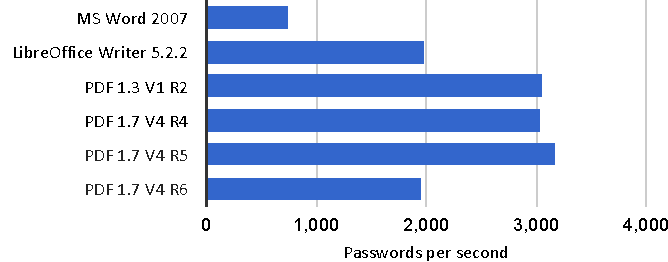
\includegraphics[width=1\textwidth]{figures/average_speed.pdf}
	\caption{Average password attempts per second}
	\label{average_speed}
\end{figure}

It should be mentioned that these results do no represent the brute-force capabilities of modern technology. Any decent tool leveraging parallelism provided by high-end GPUs will most probably achieve better results in terms of performance. Further work may include implementing such tools as clients for our distributed password recovery system. 

\chapter{Conclusion}

The aim of this thesis was to discuss and evaluate protection mechanisms offered by widely used electronic document formats. The evaluated formats are Microsoft Office documents, Portable Document Format (PDF) and Open Document Format.  The main focus was on mechanisms providing confidentiality, commonly ensured by document encryption. 

The first part provides a necessary insight into the relevant parts of the document format specifications. Furthermore, design decisions and their implications are discussed. The level of detail is chosen, to provide relevant knowledge to the reader without the need to study the corresponding specifications in depth.

The main benefit is the created distributed password recovery system. The system in its current state was used to evaluate the effectiveness of today protection mechanism used by the discussed document formats. Focus on modularity and extensibility ensure that further modifications to the system, may greatly improve the system's capabilities and usability. As an example, two proposed improvements are implementing dictionary based password guessing and support for fast and openly available brute-force tools, such as hashcat or John The Ripper.

\bibliography{thesis} 
\inputencoding{utf8}
\bibliographystyle{ieeetr}

\begin{appendix}
	\chapter{Attachements}
	\section{[MS-OFFCRYPTO] Structures and Schemas}
	\textbf{EncryptionInfo Stream (Agile Encryption) Schema}\label{ei_agile_stream}
	\begin{lstlisting}
<?xml version="1.0" encoding="utf-8"?>
<xs:schema attributeFormDefault="unqualified" elementFormDefault="qualified"
    targetNamespace="http://schemas.microsoft.com/office/2006/encryption"
    xmlns="http://schemas.microsoft.com/office/2006/encryption"
    xmlns:xs="http://www.w3.org/2001/XMLSchema">
  <xs:simpleType name="ST_SaltSize">
    <xs:restriction base="xs:unsignedInt">
      <xs:minInclusive value="1" />
      <xs:maxInclusive value="65536" />
    </xs:restriction> 
  </xs:simpleType> 
  <xs:simpleType name="ST_BlockSize">
    <xs:restriction base="xs:unsignedInt">
      <xs:minInclusive value="2" /> 
      <xs:maxInclusive value="4096" />
    </xs:restriction> 
  </xs:simpleType> 
  <xs:simpleType name="ST_KeyBits"> 
    <xs:restriction base="xs:unsignedInt"> 
      <xs:minInclusive value="8" /> 
    </xs:restriction> 
  </xs:simpleType> 
  <xs:simpleType name="ST_HashSize"> 
    <xs:restriction base="xs:unsignedInt">
      <xs:minInclusive value="1" /> 
      <xs:maxInclusive value="65536" /> 
    </xs:restriction> 
  </xs:simpleType> 
  <xs:simpleType name="ST_SpinCount"> 
    <xs:restriction base="xs:unsignedInt"> 
      <xs:minInclusive value="0" /> 
      <xs:maxInclusive value="10000000" /> 
    </xs:restriction>
  </xs:simpleType> 
  <xs:simpleType name="ST_CipherAlgorithm"> 
    <xs:restriction base="xs:string"> 
      <xs:minLength value="1" /> 
    </xs:restriction> 
  </xs:simpleType>
  <xs:simpleType name="ST_CipherChaining"> 
    <xs:restriction base="xs:string"> 
      <xs:minLength value="1" /> 
    </xs:restriction> 
  </xs:simpleType> 
  <xs:simpleType name="ST_HashAlgorithm"> 
    <xs:restriction base="xs:string"> 
      <xs:minLength value="1" /> 
    </xs:restriction> 
  </xs:simpleType>
  <xs:complexType name="CT_KeyData"> 
    <xs:attribute name="saltSize" type="ST_SaltSize" 
       use="required" /> 
    <xs:attribute name="blockSize" type="ST_BlockSize"
       use="required" /> 
    <xs:attribute name="keyBits" type="ST_KeyBits"
       use="required" /> 
    <xs:attribute name="hashSize" type="ST_HashSize"
       use="required" /> 
    <xs:attribute name="cipherAlgorithm" 
       type="ST_CipherAlgorithm" use="required" /> 
    <xs:attribute name="cipherChaining"
       type="ST_CipherChaining" use="required" /> 
    <xs:attribute name="hashAlgorithm" type="ST_HashAlgorithm"
       use="required" /> 
    <xs:attribute name="saltValue" type="xs:base64Binary" 
       use="required" /> 
  </xs:complexType>
  <xs:complexType name="CT_DataIntegrity"> 
    <xs:attribute name="encryptedHmacKey" 
                  type="xs:base64Binary" use="required" /> 
    <xs:attribute name="encryptedHmacValue" 
                  type="xs:base64Binary" use="required" /> 
  </xs:complexType>
  <xs:complexType name="CT_KeyEncryptor"> 
    <xs:sequence>
      <xs:any processContents="lax" /> 
    </xs:sequence>
    <xs:attribute name="uri" type="xs:token" /> 
  </xs:complexType>
  <xs:complexType name="CT_KeyEncryptors"> 
    <xs:sequence>
      <xs:element name="keyEncryptor" type="CT_KeyEncryptor" minOccurs="1" maxOccurs="unbounded" /> 
    </xs:sequence>
  </xs:complexType>
  <xs:complexType name="CT_Encryption"> 
    <xs:sequence>
      <xs:element name="keyData" type="CT_KeyData" 
          minOccurs="1" maxOccurs="1" /> 
      <xs:element name="dataIntegrity" type="CT_DataIntegrity" 
          minOccurs="0" maxOccurs="1" /> 
      <xs:element name="keyEncryptors" type="CT_KeyEncryptors"
          minOccurs="1" maxOccurs="1" /> 
    </xs:sequence>
  </xs:complexType>
  <xs:element name="encryption" type="CT_Encryption" /> 
</xs:schema>
	\end{lstlisting}
\textbf{PasswordKeyEncryptor Schema}\label{ei_password_encryptor}
	\begin{lstlisting}
<?xml version="1.0" encoding="utf-8"?>
  <xs:schema attributeFormDefault="unqualified" elementFormDefault="qualified" targetNamespace="http://schemas.microsoft.com/office/2006/keyEncryptor/password" xmlns="http://schemas.microsoft.com/office/2006/keyEncryptor/password" xmlns:e="http://schemas.microsoft.com/office/2006/encryption" xmlns:xs="http://www.w3.org/2001/XMLSchema"> 
  <xs:import namespace="http://schemas.microsoft.com/office/2006/encryption" schemaLocation="encryptionInfo.xsd" /> 
  <xs:simpleType name="ST_PasswordKeyEncryptorUri"> 
    <xs:restriction base="xs:token">
      <xs:enumeration value="http://schemas.microsoft.com/office/2006/keyEncryptor/password" />
    </xs:restriction>
  </xs:simpleType> 
  <xs:complexType name="CT_PasswordKeyEncryptor">
    <xs:attribute name="saltSize" type="e:ST_SaltSize" 
       use="required" />
    <xs:attribute name="blockSize" type="e:ST_BlockSize" 
       use="required" /> 
    <xs:attribute name="keyBits" type="e:ST_KeyBits" 
       use="required" />
    <xs:attribute name="hashSize" type="e:ST_HashSize" 
       use="required" /> 
    <xs:attribute name="cipherAlgorithm" 
       type="e:ST_CipherAlgorithm" use="required" /> 
    <xs:attribute name="cipherChaining"
       type="e:ST_CipherChaining" use="required" /> 
    <xs:attribute name="hashAlgorithm" 
       type="e:ST_HashAlgorithm" use="required" /> 
    <xs:attribute name="saltValue" type="xs:base64Binary" 
       use="required" /> 
    <xs:attribute name="spinCount" type="e:ST_SpinCount"
       use="required" />
    <xs:attribute name="encryptedVerifierHashInput"
       type="xs:base64Binary" use="required" /> 
    <xs:attribute name="encryptedVerifierHashValue"
       type="xs:base64Binary" use="required" />
    <xs:attribute name="encryptedKeyValue"
       type="xs:base64Binary" use="required" />
  </xs:complexType> 
  <xs:element name="encryptedKey" 
       type="CT_PasswordKeyEncryptor" />
</xs:schema>
	\end{lstlisting}
\end{appendix}
\end{document}

